%!TEX root = ../Main.tex

\chapter{PolyMarker: A fast polyploid primer design pipeline}
\chaptermark{PolyMarker}
%\section{Introduction} 
%Explain how the SNP markers are designed without the tool and an overview. 
One of the main challenges of working with polyploid species is the design of genome specific molecular markers. 
This is particularly true when targeting conserved homoeologue regions, where a primer could bind to a pair,or triplet, of identical sequences. 
For that reason, designing primers for polyploids require to include bases that are specific to the target, in addition to the physicochemical properties of the primer.  
The traditional methodology to find primer candidates include a blast search and a local alignment, select the primer candidates manually, and finally, validate the primers with a tool, like \verb|Primer3| \citep{Rozen}. 
To reduce the time invested in designed primers I have developed PolyMarker \citep{Ramirez-Gonzalez2015a}, a pipeline to automate the primer design for polyploid organisms.  

\section{Pipeline}

\begin{figure}
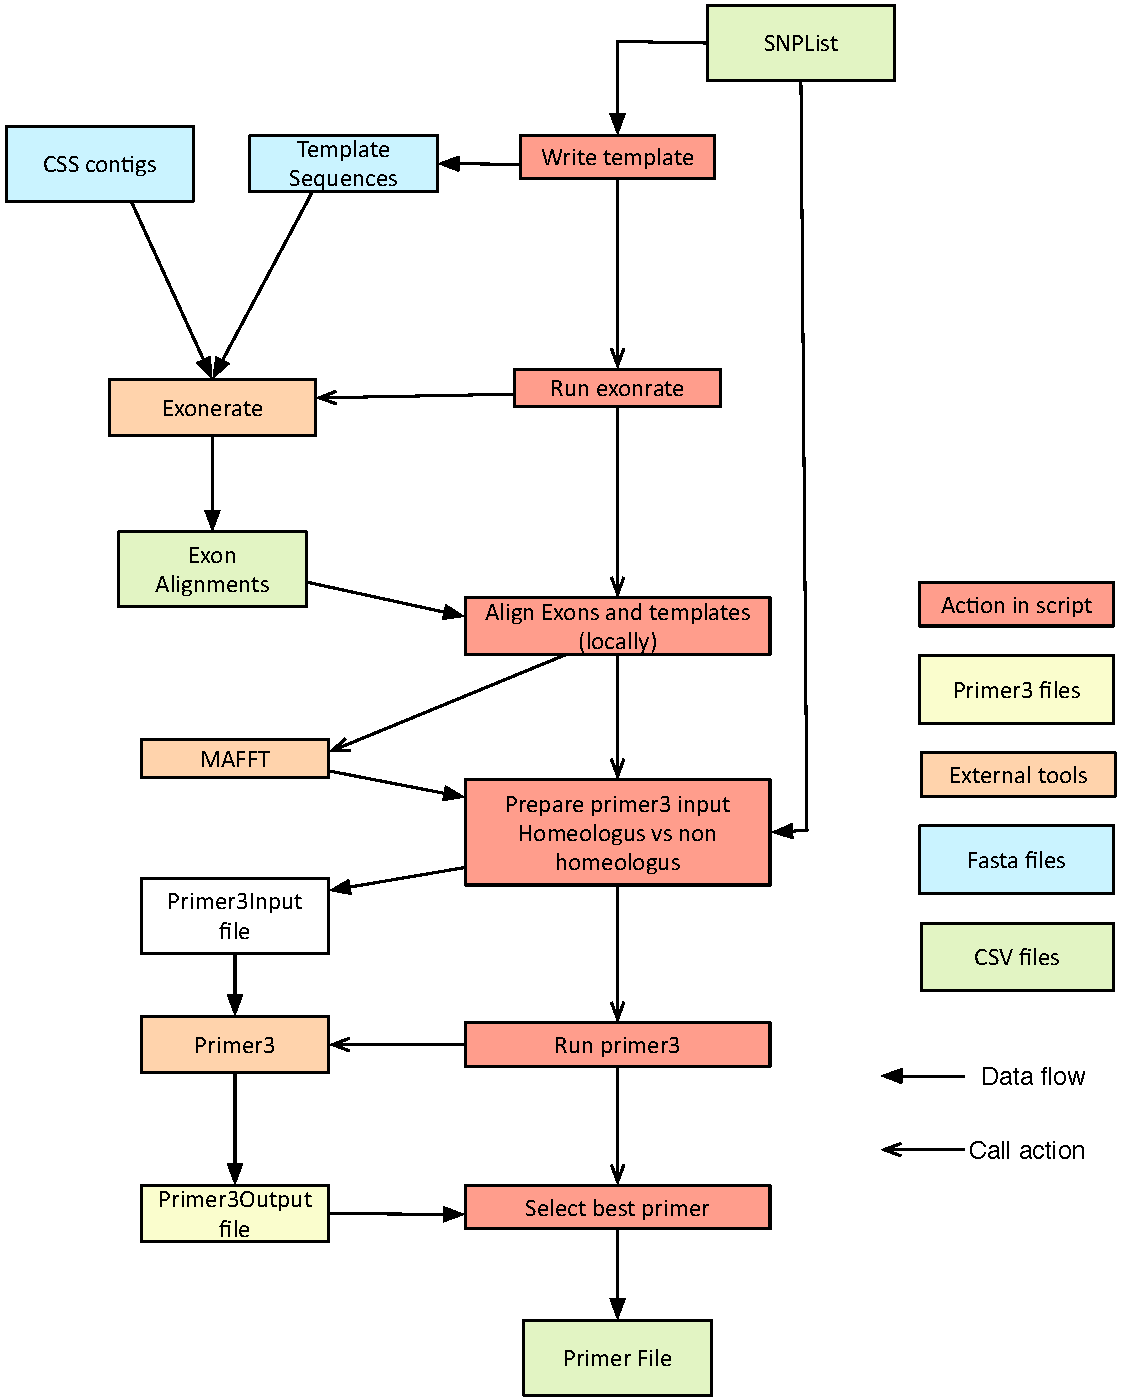
\includegraphics[width=1\textwidth]{PolyMarker/Figures/pipeline.pdf}
        \caption{Steps and tools called by PolyMarker. The colour of the boxes represent: the step is an action inside the script(red); actions of the script(orange); temporary files(yellow); inputs(blue) and; outpus(green)}
        \label{fig:poly:pipeline}
\end{figure}

PolyMarker is an automated pipeline that takes as input a list of SNPs and a reference file and produces a list of primer triplets for SNP genotyping. 
The list of SNPs is first converted to a \verb|FASTA| file with ambiguity codes \citep{Cornish-Bowden1985} 
The template sequences are aligned with \verb|exonerate| \citep{Slater2005}  to find the homoeologous regions to the target sequence. 
Then, the alignment between homoeologues is refined using \verb|MAFFT| \citep{Katoh2013}. 
A list of candidate variations is produced and used as input for \verb|Primer3| \citep{Rozen}. 
Finally, the output of \verb|Primer3| is parsed to find the best primer pair that contains a the targeted SNP and a base that is specific to the target genome (Figure \ref{fig:poly:pipeline}).  
The pipeline is written as a Ruby script, using parsers and wrappers from BioRuby \citep{Goto2010} and bio-samtools \citep{Etherington2015,Ramirez-Gonzalez2012}. 
The software is open source and released as a biogem \citep{Bonnal2012}, \verb|bio-polyploid-tools|, the source code is available in github: \verb|https://github.com/TGAC/bioruby-polyploid-tools|.


The PolyMarker input consist on SNP list with: unique name for the marker, the target chromosome and the sequence for the marker. 
The alternative alleles are surrounded by square brackets within the sequence. PolyMarker can take a list of several markers and design them in batch, Figure \ref{fig:poly:input}. 
A \verb|FASTA| file is produced with all the template sequences, with the alternative alleles substituted by the IUAPC ambiguity codes \citep{Cornish-Bowden1985}. 
The flanking sequence surrounding the SNP is limited by default to 100bp to reduce the search time and avoid missing regions that diverge near the SNP, as when the variation is near an intron-exon junction. 
%%TODO: Should we elaborate more here? 

\begin{figure}
    \centering
    \begin{subfigure}[b]{0.8\textwidth}
        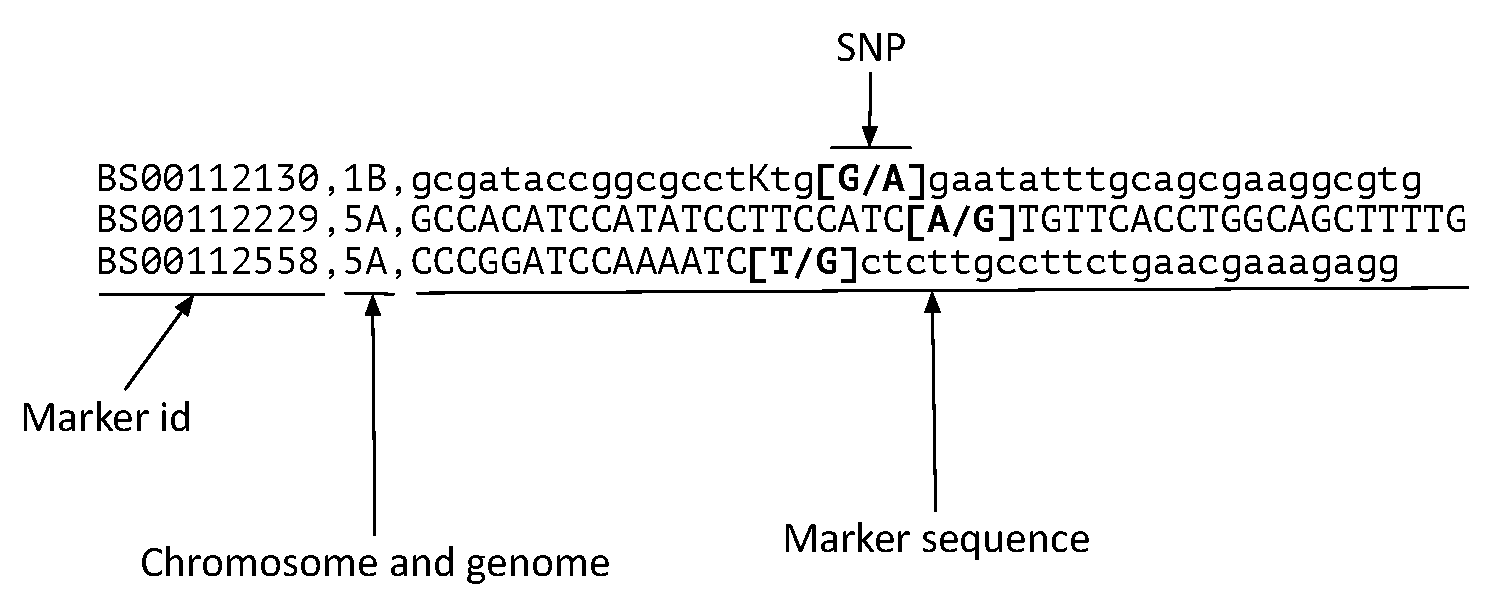
\includegraphics[width=1\textwidth]{PolyMarker/Figures/aln/input.pdf} 
        \caption{}
        \label{fig:poly:input}
    \end{subfigure}

    \begin{subfigure}[b]{0.4\textwidth}
        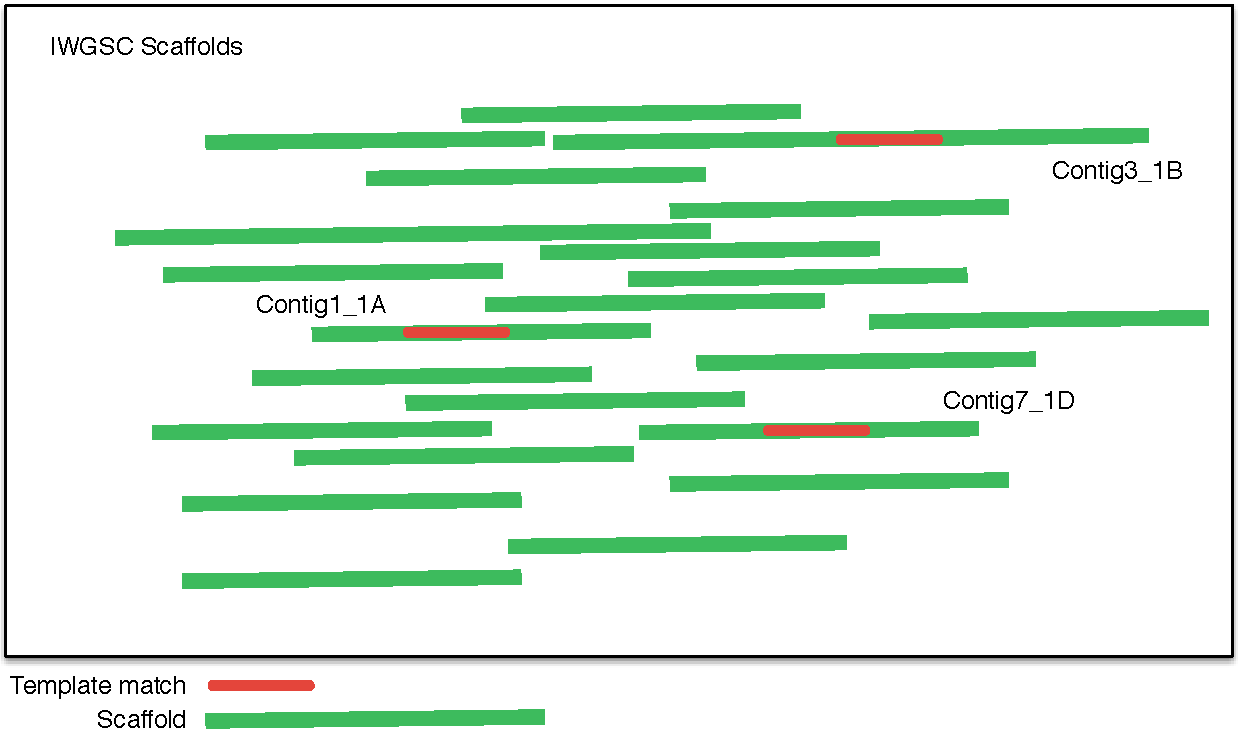
\includegraphics[width=1\textwidth]{PolyMarker/Figures/aln/scaffoldsSearch.pdf}
        \caption{}
        \label{fig:poly:globalSearch}
    \end{subfigure}
    ~ %add desired spacing between images, e. g. ~, \quad, \qquad, \hfill etc. 
      %(or a blank line to force the subfigure onto a new line)
    \begin{subfigure}[b]{0.4\textwidth}
        \raisebox{10mm} { 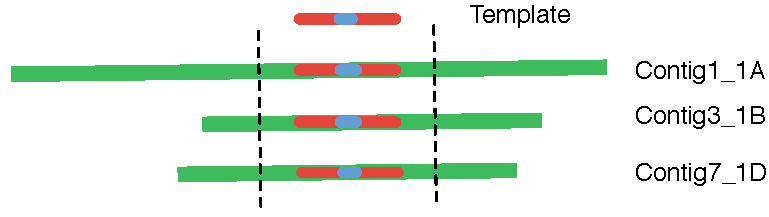
\includegraphics[width=1\textwidth]{PolyMarker/Figures/aln/scaffoldsFoundAround.pdf} }
        \caption{}
        \label{fig:poly:globalAround} 
    \end{subfigure}
    
    \begin{subfigure}[b]{0.4\textwidth}
        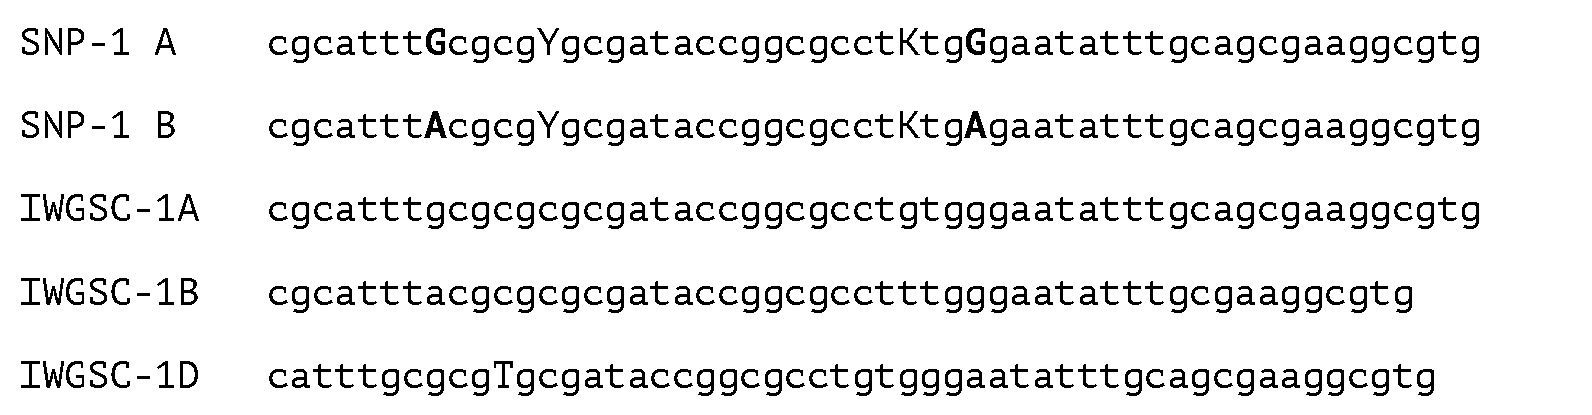
\includegraphics[width=1\textwidth]{PolyMarker/Figures/aln/scaffoldsFound.pdf}
        \caption{}
        \label{fig:poly:globalSequence}
    \end{subfigure}
    ~ %add desired spacing between images, e. g. ~, \quad, \qquad, \hfill etc. 
      %(or a blank line to force the subfigure onto a new line)
    \begin{subfigure}[b]{0.4\textwidth}
        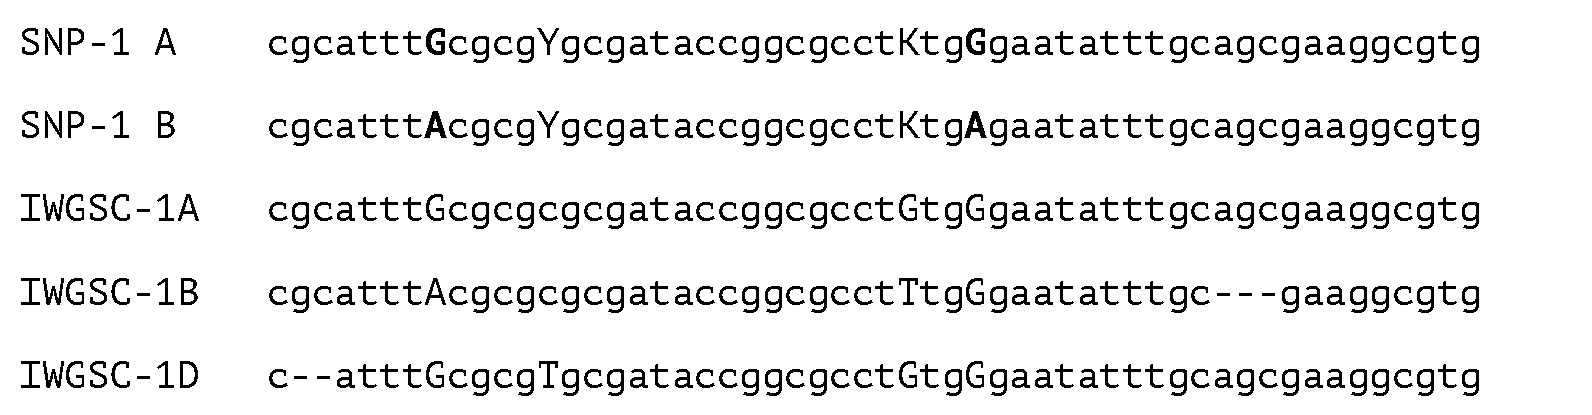
\includegraphics[width=1\textwidth]{PolyMarker/Figures/aln/localAlignment.pdf} 
        \caption{}
        \label{fig:poly:localSequence}
    \end{subfigure}

    \begin{subfigure}[b]{0.8\textwidth}
        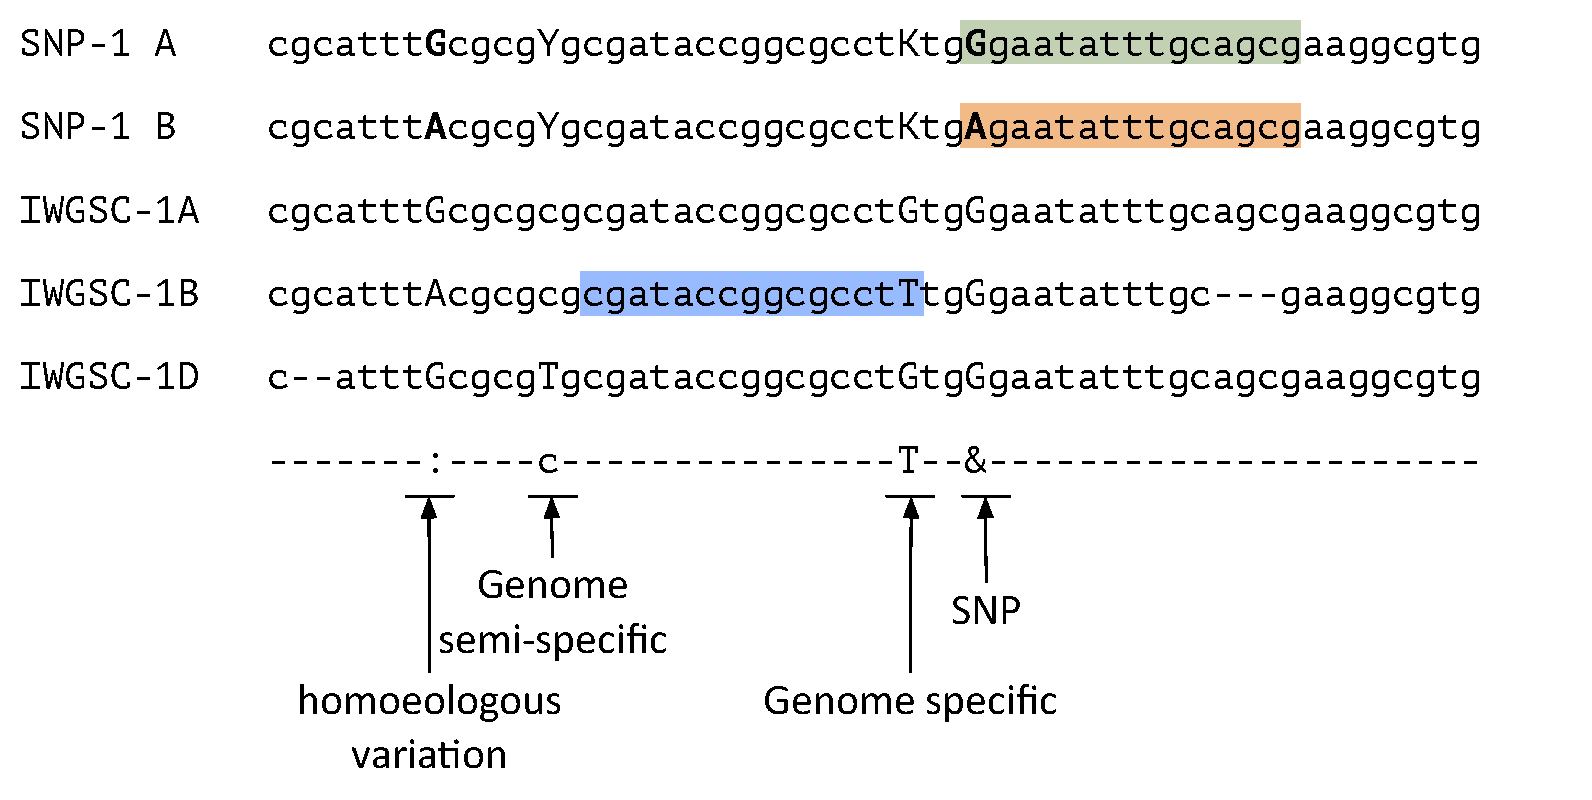
\includegraphics[width=1\textwidth]{PolyMarker/Figures/aln/mask.pdf} 
        \caption{}
        \label{fig:poly:mask}
    \end{subfigure}
    \caption{Alignments done by PolyMarker.(\subref{fig:poly:input}) input. The alternative alleles are sorrounded by brackets. (\subref{fig:poly:globalSearch}) Global search of templates in the reference contigs. (\subref{fig:poly:globalAround}) Selected regions around the SNP on every chromosome. (\subref{fig:poly:globalSequence}) Sequence of found regions around the SNP. (\subref{fig:poly:localSequence}) Local alignment on regions around the SNP detects indels. (\subref{fig:poly:mask}) Alignment with mask and primer candidates.}
    \label{fig:global}
\end{figure}

The template sequences are aligned to the reference using \verb|exonerate| \citep{Slater2005}, Figure \ref{fig:poly:globalSearch}. 
The alignment is refined with the \verb|--model est2genome| option, to allow the search of sequences coming from transcripts, a common source of SNPs \citep{Allen2011}. 
The exonerate output is formatted with the \verb|--ryo| (roll your own format) to get an output easy to parse. 
All the hits that contain the SNP are extracted from the reference with a flanking sequence that extend out of the hit, by defualt, to 100bp on each side of the SNP, Figure \ref{fig:poly:globalAround}.
The size of the flanking sequence can be set to different sizes to allow the design of different types of primers. 
Different homoeologues may contain small indels, Figure \ref{fig:poly:globalSequence}. 
To enable a comparasion base-per-base, a local alignment with \verb|MAFFT| \citep{Katoh2013} is produced, Figure \ref{fig:poly:localSequence}. 

PolyMarker searches across each base in the local alignment to identify the variations across homoeologues and the target marker.
A mask is produced to highlight the bases with a variations, Figure \ref{fig:poly:mask}, on the following categories:
\begin{labeling}{Non-homoeologous}
%\begin{description}[align=right,labelwidth=4cm]
\item [Specific] Homoeologous polymorphism which is only present in the target genome (upper case).
\item [Semi-specific] Homoeologous polymorphism which is found in 2 of the 3 genomes, hence it discriminates against one of the off-target genomes or when not all the homoeologous sequences were found (lower case).
\item [Non-specific] No variation is found across homoeologues (\texttt{-}).
\item [Homoeologous] The target SNP is present across different chromosomes, so candidate SNP markers on this category are not expected to be reliably identify the allele (\texttt{:}).
\item [Non-homoeologous] The target SNP is not present across chromosomes, so it can be used to identify an allele (\texttt{\&}).
%\end{description} 
\end{labeling} 

PolyMarker was designed to produce SNP assays for KASP genotyping \citep{LGC}, which requires a common primer and two allele-specific primers. 
The common primer is selected to start on a position from a: Specific; Semi-specific or; Non-specific, on that priority. 
This means that the common primer will be as specific as possible in the region. 
For the allele-specific primers, the starting position of the primer is on the base with the SNP. 
To ensure that the stability of the candidate primers will be met, the putative starting positions are tested with \texttt{Primer3} \citep{Rozen}. 

%%TODO: check for 3primer/ 5 primer instead of starts 
PolyMarker was designed and validated with the markers described in section \ref{yr15:geneticMap}. 
For wheat, PolyMarker uses the contigs from \cite{Mayer2014}, as deposited in Ensembl. 
As new releases of the wheat genome are made available, different parsers to assign the chromosome to each sequence can be added with little effort to PolyMarker. 




\section{Applications of PolyMarker}

PolyMarker is not restricted to wheat or to KASP assays, the source code is flexible and can be extended for other types of analysis. 
On each of the following projects, PolyMarker has been adapted to design primers in species where KASP hasn't been used before, the primers are used for regular PCR amplification, or the use of KASP is not the conventional SNP calling. 

\subsection{KASP assays for public sets of SNPs} 

PolyMarker was used to design KASP assays for the 81,587 markers from \citep{Wang2014}, available on the PolyMarker website and in CeralsDB \citep{Wilkinson2012}. 
Of those markers, 40,267 where designed using the target chromosome using the genetic map published by the genetic map. 
Genes without a genetic position were aligned to scaffolds sorted by chromosome from the International Wheat Genome Sequencing Consortium \citep{Mayer2014} with BLAT \citep{Kent2002} and the best hit was selected as putative location. 
97.5\% of the assays where designed and 76\% of them are semi-specific or specific, thereby improving their expected performance with respect to randomly designed primers (Table \ref{tab:poly:designed}). 
A subset of the designed assay was used to genotype a mapping population to find resistance to Fusarium head blight \citep{Burt2015}. 

\subsection{SNPs in a mutant population}

PolyMarker was used to design primers to validate SNPs in a Targeted Induced Local Lesions in Genomes (TILLING) population, an approach to identify the function of genes by mutating them. 
To calibrate the SNP calling, KASP assays were designed to get the mutations from $M_{2}$, $M_{3}$ and, $M_{5}$ mutants \citep{King2015}. 
%TODO: Add more details as suplemental?
Then primers were designed for the whole mutant population, consisting of 1,200 Cadenza (Hexaploid) and 1,535 Kronos (Tetraploid) wheat lines \citep{Krasileva2016}. Genome-specific primers  172 and 80 SNP assays on 19 and 8 $M_{4}$ Cadenza and Kronos lines respectively. 
Of those, 71(85.5\%) Kronos and 147(88.8\%) of the Cadenza primers where valid assays (Tables \ref{app:PolyMarkerM4ValidationCadenza} and \ref{app:PolyMarkerM4ValidationKronos}).  

\subsection{Deletions on a mutant population}
%Algorithm to produce KASP for deletions in polyploids. 

\begin{figure}
    \centering
    \begin{subfigure}[b]{0.45\textwidth}
        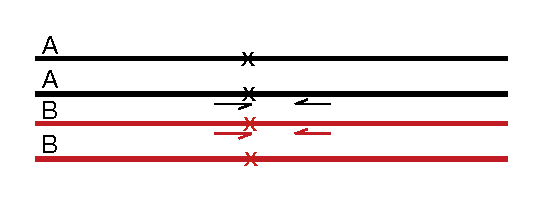
\includegraphics[width=1\textwidth]{PolyMarker/Figures/deletions/wt.pdf}
        \caption{}
        \label{fig:poly:wt}
    \end{subfigure}
    ~
     \begin{subfigure}[b]{0.45\textwidth}
        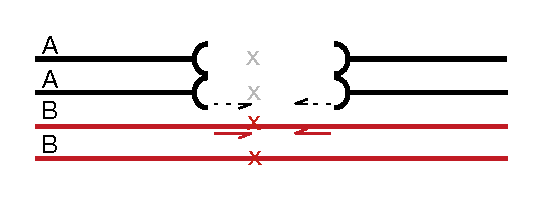
\includegraphics[width=1\textwidth]{PolyMarker/Figures/deletions/homM4.pdf}
        \caption{}
        \label{fig:poly:homM4}
    \end{subfigure}
    \begin{subfigure}[b]{0.3\textwidth}
        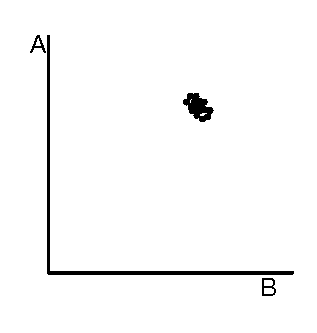
\includegraphics[width=1\textwidth]{PolyMarker/Figures/deletions/homFalse.pdf} 
        \caption{}
        \label{fig:poly:homFalse}
    \end{subfigure}
    ~
    \begin{subfigure}[b]{0.3\textwidth}
        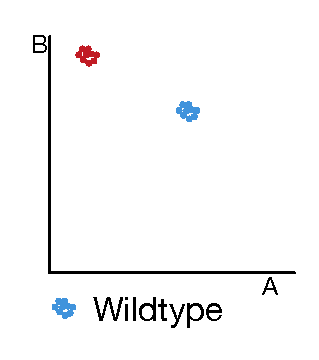
\includegraphics[width=1\textwidth]{PolyMarker/Figures/deletions/homReal.pdf}
        \caption{}
        \label{fig:poly:homReal}
    \end{subfigure}
    \caption{KASP assays to validate homozygous deletions. (\subref{fig:poly:wt}) Primer positions for wildtype. (\subref{fig:poly:homM4}) Primer positions on  homozygous deletion on $M_{4}$ (\subref{fig:poly:homFalse} Heterozygous amplification on wildtype, including both homoeologues. (\subref{fig:poly:homReal}) Homozygous amplification on deletion line, only the non-deletad homoeologue is amplified. }
\end{figure}

On some of the TILLING mutant lines long deletions were detected \citep{Krasileva2016}.
To validate the deletions is possible to use KASP assays to produce primers that amplify homoeologues.  
PolyMarker was modified to search for variations across homoeologues to select a common primer that will amplify two genomes, Figures \ref{fig:poly:wt} and \ref{fig:poly:homM4}. 
On lines without the targeted deletion, the amplification correspond to an homozygous assay, Figure \ref{fig:poly:homFalse}.  
When a deletion is present the results of the assay look like an homozygous sample, with the intensity of the assay towards the the conserved homoeologue, Figure \ref{fig:poly:homReal}.
A set of KASP assays for the the deletions and mutations located on the same chromosome where designed to validate 11 homozygous deletions on $m_{4}$ plants. 
In all cases the segregation of the mutiations was as expected, except for a predicted heterozygous mutation that was called as homozygous. 
Also, all the KASP assays that contained a deletion were called homozygous, as expected. 
To ensure that the calls didn't come from a single cluster, 4 wildtype plants were genotyped and the markers for deletions where called as heterozygous. 
An example of a validated deletion, with the calls for each individual is shown on Table \ref{app:poly:homDelCad0423}.

\subsection{PolyMarker public web service}
To make PolyMarker accessible to the community, a web server that allow the submission of SNPs was developed. 
The web interface consists on two virtual machines, one with a web facing interface that stores the queries, and a dedicated node to submit jobs to an HPC cluster.
The on-line interface further simplifies the design of KASP assays, a process that used to take a couple of weeks now is done in a couple of hours. 
Since the release of the public service in July 2014 until August 2016, 1,739 requests to PolyMarker have been done. 
%TODO: Does this sounds like too much marketing? 


\subsection{Genotyping of \textit{Puccinia 
striiformis} f. sp. \textit{tritici} isolates.}
In \cite{Hubbard2015}, \textit{Puccinia striiformis} f. sp. \textit{tritici} (PST) isolates were sequenced and assigned to clusters, according to their genotype.
The clusters are useful to monitor the changes in the pathogen population, which can be used to predict if certain wheat lines will be resistant to the isolates in the field. 
PolyMarker was used to design primers for PST, using the assembly PST-130 \citep{Cantu2011}.
Out of 15 assays 11 can be used to identify to which cluster of isolates a sample is likely to belong, Supplemental Table \ref{app:PolyMarkerPST}.


\section{Discussion}

PolyMarker is a tool that was born as part of the validation of the SNPs found in Chapter \ref{yr15}. 
Originally, the primer design was ought to be done manually, a slow, error-prone and, repetitive process. 
The steps require the use of several bioinformatics tools, but once I figured out the steps I decided to automate the process. 
Since designing genome-specific primers is a common task in wheat research and breeding, the community showed interest on the tool and I decided to refine it and make it open source. 
PolyMarker has been used successfully in several projects and it even allowed the novel use of KASP assays to validate long deletions in polyploids. 

The current web interface of PolyMarker is limited to KASP assays, however the command line version is more flexible and has been used to design primers for PCR amplicons, capillary sequencing and on other organisms. 
The ideas behind PolyMarker had been taken by other projects like the scripts described in \cite{Ma2015} and the corresponding web interface, GSP \citep{Wang2016}. 
As new references of wheat come available, PolyMarker should be updated to work with pseudomolecules and the web interface updated accordingly.  

%Remarks on the importance of getting the primers right, and the time saved by automating the primer selection. Also mention other primer design tools that have been inspired by polymarker: \cite{Ma2015}, \cite{Wang2016}

 


